%% LyX 2.3.6.2 created this file.  For more info, see http://www.lyx.org/.
%% Do not edit unless you really know what you are doing.
\documentclass[english]{beamer}
\usepackage[T1]{fontenc}
\usepackage[latin9]{inputenc}
\setcounter{secnumdepth}{3}
\setcounter{tocdepth}{3}
\usepackage{babel}
\usepackage{amstext}
\usepackage{graphicx}
\usepackage[all]{xy}
\ifx\hypersetup\undefined
  \AtBeginDocument{%
    \hypersetup{unicode=true,pdfusetitle,
 bookmarks=true,bookmarksnumbered=false,bookmarksopen=false,
 breaklinks=false,pdfborder={0 0 1},backref=false,colorlinks=true}
  }
\else
  \hypersetup{unicode=true,pdfusetitle,
 bookmarks=true,bookmarksnumbered=false,bookmarksopen=false,
 breaklinks=false,pdfborder={0 0 1},backref=false,colorlinks=true}
\fi

\makeatletter
%%%%%%%%%%%%%%%%%%%%%%%%%%%%%% Textclass specific LaTeX commands.
% this default might be overridden by plain title style
\newcommand\makebeamertitle{\frame{\maketitle}}%
% (ERT) argument for the TOC
\AtBeginDocument{%
  \let\origtableofcontents=\tableofcontents
  \def\tableofcontents{\@ifnextchar[{\origtableofcontents}{\gobbletableofcontents}}
  \def\gobbletableofcontents#1{\origtableofcontents}
}
\newenvironment{lyxcode}
  {\par\begin{list}{}{
    \setlength{\rightmargin}{\leftmargin}
    \setlength{\listparindent}{0pt}% needed for AMS classes
    \raggedright
    \setlength{\itemsep}{0pt}
    \setlength{\parsep}{0pt}
    \normalfont\ttfamily}%
   \def\{{\char`\{}
   \def\}{\char`\}}
   \def\textasciitilde{\char`\~}
   \item[]}
  {\end{list}}

%%%%%%%%%%%%%%%%%%%%%%%%%%%%%% User specified LaTeX commands.
\usetheme[secheader]{Boadilla}
\usecolortheme{seahorse}
\title[Relational parametricity]{Relational parametricity and "theorems for free"}
\subtitle{A tutorial, with example code in Scala}
\author{Sergei Winitzki}
\date{2021-09-04}
\institute[ABTB]{Academy by the Bay}
\setbeamertemplate{headline}{} % disable headline at top
\setbeamertemplate{navigation symbols}{} % disable navigation bar at bottom
\usepackage[all]{xy} % xypic
%\makeatletter
% Macros to assist LyX with XYpic when using scaling.
\newcommand{\xyScaleX}[1]{%
\makeatletter
\xydef@\xymatrixcolsep@{#1}
\makeatother
} % end of \xyScaleX
\makeatletter
\newcommand{\xyScaleY}[1]{%
\makeatletter
\xydef@\xymatrixrowsep@{#1}
\makeatother
} % end of \xyScaleY

% Double-stroked fonts to replace the non-working \mathbb{1}.
\usepackage{bbold}
\DeclareMathAlphabet{\bbnumcustom}{U}{BOONDOX-ds}{m}{n} % Use BOONDOX-ds or bbold.
\newcommand{\custombb}[1]{\bbnumcustom{#1}}
% The LyX document will define a macro \bbnum{#1} that calls \custombb{#1}.

\usepackage{relsize} % make math symbols larger or smaller
\usepackage{stmaryrd} % some extra symbols such as \fatsemi
% Note: using \forwardcompose inside a \text{} will cause a LaTeX error!
\newcommand{\forwardcompose}{\hspace{1.5pt}\ensuremath\mathsmaller{\fatsemi}\hspace{1.5pt}}


% Make underline green.
\definecolor{greenunder}{rgb}{0.1,0.6,0.2}
%\newcommand{\munderline}[1]{{\color{greenunder}\underline{{\color{black}#1}}\color{black}}}
\def\mathunderline#1#2{\color{#1}\underline{{\color{black}#2}}\color{black}}
% The LyX document will define a macro \gunderline{#1} that will use \mathunderline with the color `greenunder`.
%\def\gunderline#1{\mathunderline{greenunder}{#1}} % This is now defined by LyX itself with GUI support.

% Scala syntax highlighting. See https://tex.stackexchange.com/questions/202479/unable-to-define-scala-language-with-listings
%\usepackage[T1]{fontenc}
%\usepackage[utf8]{inputenc}
%\usepackage{beramono}
%\usepackage{listings}
% The listing settings are now supported by LyX in a separate section "Listings".
\usepackage{xcolor}

\definecolor{scalakeyword}{rgb}{0.16,0.07,0.5}
\definecolor{dkgreen}{rgb}{0,0.6,0}
\definecolor{gray}{rgb}{0.5,0.5,0.5}
\definecolor{mauve}{rgb}{0.58,0,0.82}
\definecolor{aqua}{rgb}{0.9,0.96,0.999}
\definecolor{scalatype}{rgb}{0.2,0.3,0.2}
\usepackage[nocenter]{qtree}
\usepackage{relsize}
\renewcommand\arraystretch{1.4}

\makeatother

\usepackage{listings}
\lstset{language=Scala,
morekeywords={{scala}},
otherkeywords={=,=>,<-,<\%,<:,>:,\#,@,:,[,],.,???},
keywordstyle={\color{scalakeyword}},
morekeywords={[2]{String,Short,Int,Long,Char,Boolean,Double,Float,BigDecimal,Seq,Map,Set,List,Option,Either,Future,Vector,Range,IndexedSeq,Try,true,false,None,Some,Left,Right,Nothing,Any,Array,Unit,Iterator,Stream}},
keywordstyle={[2]{\color{scalatype}}},
frame=tb,
aboveskip={1.5mm},
belowskip={0.5mm},
showstringspaces=false,
columns=fullflexible,
keepspaces=true,
basicstyle={\smaller\ttfamily},
extendedchars=true,
numbers=none,
numberstyle={\tiny\color{gray}},
commentstyle={\color{dkgreen}},
stringstyle={\color{mauve}},
frame=single,
framerule={0.0mm},
breaklines=true,
breakatwhitespace=true,
tabsize=3,
framexleftmargin={0.5mm},
framexrightmargin={0.5mm},
xleftmargin={1.5mm},
xrightmargin={1.5mm},
framextopmargin={0.5mm},
framexbottommargin={0.5mm},
fillcolor={\color{aqua}},
rulecolor={\color{aqua}},
rulesepcolor={\color{aqua}},
backgroundcolor={\color{aqua}},
mathescape=false,
extendedchars=true}
\renewcommand{\lstlistingname}{Listing}

\begin{document}
\global\long\def\gunderline#1{\mathunderline{greenunder}{#1}}%
\global\long\def\bef{\forwardcompose}%
\global\long\def\bbnum#1{\custombb{#1}}%
\frame{\titlepage}
\begin{frame}{Motivation for parametricity. ``Theorems for free''}

\textbf{Parametricity}: all fully parametric functions satisfy their
naturality laws
\begin{itemize}
\item Naturality law: code must work in the same way for all types
\end{itemize}
\begin{lyxcode}
\textcolor{blue}{\small{}def~headOption{[}A{]}:~List{[}A{]}~=>~Option{[}A{]}~=~\{}{\small\par}

\textcolor{blue}{\small{}~~case~Nil~~~~~~~~~~~~=>~None}{\small\par}

\textcolor{blue}{\small{}~~case~head~::~tail~~~=>~Some(head)}{\small\par}

\textcolor{blue}{\small{}\}}{\small\par}
\end{lyxcode}
\begin{itemize}
\item \textbf{``Fully parametric''} code: use only type parameters, no
JVM reflection 
\begin{itemize}
\item Naturality laws are ``for free'' only if all code is fully parametric
\end{itemize}
\item Naturality law for \texttt{\textcolor{blue}{\small{}headOption}}:
for any \texttt{\textcolor{blue}{\small{}x:~List{[}A{]}}} and \texttt{\textcolor{blue}{\small{}f:~A
=> B}},
\end{itemize}
\begin{lyxcode}
\textcolor{blue}{\small{}headOption(x).map(f)~==~headOption(x.map(f))}{\small\par}
\end{lyxcode}
Parametricity theorems work only if the code is ``fully parametric''

Parametricity theorems apply only to a subset of a programming language
\begin{itemize}
\item Usually, it is a certain flavor of typed lambda calculus
\end{itemize}
\end{frame}

\begin{frame}{Examples of code that fails parametricity}

Explicit matching on type parameters using JVM reflection:
\begin{lyxcode}
\textcolor{blue}{\small{}def~badHeadOpt{[}A{]}:~List{[}A{]}~=>~Option{[}A{]}~=~\{}{\small\par}

\textcolor{blue}{\small{}~~case~Nil~~~~~~~~~~~~~~~~~=>~None}{\small\par}

\textcolor{blue}{\small{}~~case~(head:~Int)~::~tail~=>~None}{\small\par}

\textcolor{blue}{\small{}~~case~head~::~tail~~~~~~~~=>~Some(head)}{\small\par}

\textcolor{blue}{\small{}\}}{\small\par}
\end{lyxcode}
Using typeclasses: define typeclass \textcolor{blue}{\small{}NotInt{[}A{]}}
returning \textcolor{blue}{\small{}true} unless \textcolor{blue}{\small{}A
= Int} 
\begin{lyxcode}
\textcolor{blue}{\small{}def~badHeadOpt{[}A{]}:~List{[}A{]}~=>~Option{[}A{]}~=~\{}{\small\par}

\textcolor{blue}{\small{}~~case~h~::~tail~if~implicitly{[}NotInt{[}A{]}{]}()~~~=>~Some(h)}{\small\par}

\textcolor{blue}{\small{}~~case~\_~=>~None}{\small\par}

\textcolor{blue}{\small{}\}}{\small\par}
\end{lyxcode}
Failure of naturality law:
\begin{lyxcode}
\textcolor{blue}{\small{}scala>~badHeadOpt(List(10,~20,~30).map(x~=>~s\textquotedbl x~=~\$x\textquotedbl ))}{\small\par}

\textcolor{blue}{\small{}res0:~Option{[}String{]}~=~Some(x~=~10)}{\small\par}

~

\textcolor{blue}{\small{}scala>~badHeadOpt(List(10,~20,~30)).map(x~=>~s\textquotedbl x~=~\$x\textquotedbl )}{\small\par}

\textcolor{blue}{\small{}res1:~Option{[}String{]}~=~None}{\small\par}
\end{lyxcode}
\end{frame}
\vspace{1\baselineskip}
~

Fully parametric programs are written using the 9 code constructions:
\begin{lstlisting}
def fmap[A, B](f: A => B): List[(A, A)] => List[(B, B)] = { // 3
   case Nil            => Nil
//   8   1                1,7 
   case head :: tail   => (f (head._1), f (head._2)) :: fmap(f)(tail)
//   8       6             2 4     6  5 2 4     6    7   9
}           // This code uses each of the nine allowed constructions.
\end{lstlisting}
\vspace{-0.2\baselineskip}

\begin{enumerate}
\item Use \lstinline!Unit! value (or equivalent type), e.g.~\lstinline!()!,
\lstinline!Nil!, \lstinline!None!
\item Use bound variable (a given argument of the function)
\item Create a function: \lstinline!{ x => expr(x) }!
\item Use a function: \lstinline!f(x)!
\item Create a product: \lstinline!(a, b)!
\item Use a product: \lstinline!p._1! (or via pattern matching)
\item Create a co-product: \lstinline!Left[A, B](x)!
\item Use a co-product: \lstinline!{ case ... => ... }! (pattern matching)
\item Use a recursive call: e.g., \lstinline!fmap(f)(tail)! within the
code of \lstinline!fmap!\medskip{}
\end{enumerate}

\begin{frame}{Why we need relational parametricity}

``Relational parametricity'' is a method for proving parametricity
theorems
\begin{itemize}
\item Main papers: \href{https://people.mpi-sws.org/~dreyer/tor/papers/reynolds.pdf}{Reynolds (1983)}
and Wadler \href{https://people.mpi-sws.org/~dreyer/tor/papers/wadler.pdf}{\textquotedblleft Theorems for free\textquotedblright}
(1989)
\begin{itemize}
\item Those papers are a bit outdated and also hard to understand 
\end{itemize}
\item There are very few pedagogical tutorials on relational parametricity
\begin{itemize}
\item ``\href{https://www.researchgate.net/publication/262348393_On_a_Relation_on_Functions}{On a relation of functions}''
by R.~Backhouse (1990) 
\item ``\href{https://themattchan.com/docs/algprog.pdf}{The algebra of programming}''
by R.~Bird and O.~de Moor (1997)
\end{itemize}
\end{itemize}
This tutorial does \emph{not} follow any of the above but derives
equivalent results
\begin{itemize}
\item Alternative approach: prove ``dinaturality'' (\href{https://www.irif.fr/~delatail/dinat.pdf}{de Lataillade},
\href{https://arxiv.org/pdf/1908.07776}{Voigtl\"ander})
\begin{itemize}
\item Dinaturality is a consequence of relational parametricity
\item In practice, dinaturality laws are sufficient in most cases
\item But some proofs still need full relational parametricity
\end{itemize}
\end{itemize}
\end{frame}

\begin{frame}{Motivating relational parametricity. I. Naturality laws}

Naturality law: applying \texttt{\textcolor{blue}{\small{}t{[}A{]}:~F{[}A{]}
=> G{[}A{]}}} \emph{before} \texttt{\textcolor{blue}{\small{}\_.map(f)}}
equals applying \texttt{\textcolor{blue}{\small{}t{[}B{]}:~F{[}B{]}
=> G{[}B{]}}} \emph{after} \texttt{\textcolor{blue}{\small{}\_.map(f)}}
for any function \texttt{\textcolor{blue}{\small{}f:~A => B}}{\small\par}

Naturality laws need \emph{lifting} \texttt{\textcolor{blue}{\small{}f:~A
=> B}} to \texttt{\textcolor{blue}{\small{}F{[}A{]} => F{[}B{]}}}
and \texttt{\textcolor{blue}{\small{}G{[}A{]} => G{[}B}}{]} 
\[
\xymatrix{\xyScaleY{2.8pc}\xyScaleX{5.5pc}\mathtt{F[A]}\ar[d]\sb(0.5){~\mathtt{\_.map(f)}\text{ for }\mathtt{F}}\ar[r]\sp(0.5){\mathtt{t[A]}} & \mathtt{G[A]}\ar[d]\sp(0.5){\mathtt{\_.map(f)}\text{ for }\mathtt{G}}\\
\mathtt{F[B]}\ar[r]\sp(0.5){\mathtt{t[B]}} & \mathtt{G[B]}
}
\]

\begin{itemize}
\item Proof of the naturality law requires induction on the code of \texttt{\textcolor{blue}{\small{}t{[}A{]}}} 
\begin{itemize}
\item This code is built up by combining the 9 code constructions
\item This code may include sub-expressions of types not covariant in \texttt{\textcolor{blue}{\small{}A}} 
\end{itemize}
\end{itemize}
\end{frame}

\begin{frame}{Motivating relational parametricity. II. The difficulty}

Cannot lift \texttt{\textcolor{blue}{\small{}f:~A => B}} to \texttt{\textcolor{blue}{\small{}F{[}A{]}
=> F{[}B{]}}} when \texttt{\textcolor{blue}{\small{}F{[}\_{]}}} is
not covariant!
\begin{itemize}
\item For covariant \texttt{\textcolor{blue}{\small{}F{[}\_{]}}} we lift
\texttt{\textcolor{blue}{\small{}f:~A => B}} to \texttt{\textcolor{blue}{\small{}fmap(f):~F{[}A{]}
=> F{[}B{]}}} 
\item For contravariant \texttt{\textcolor{blue}{\small{}F{[}\_{]}}} we
lift \texttt{\textcolor{blue}{\small{}f:~B => A}} to \texttt{\textcolor{blue}{\small{}cmap(f):~F{[}A{]}
=> F{[}B{]}}} 
\end{itemize}
In general, \texttt{\textcolor{blue}{\small{}F{[}\_{]}}} will be neither
covariant nor contravariant
\begin{itemize}
\item Example: \texttt{\textcolor{blue}{\small{}foldLeft}} with respect
to type parameter \texttt{\textcolor{blue}{\small{}A}} 
\end{itemize}
\begin{lyxcode}
\textcolor{blue}{\small{}def~foldLeft{[}T,~A{]}:~List{[}T{]}~=>~(T~=>~A~=>~A)~=>~A~=>~A}{\small\par}
\end{lyxcode}
\begin{itemize}
\item This is \emph{not} of the form \texttt{\textcolor{blue}{\small{}F{[}A{]}
=> G{[}A{]}}} with covariant \texttt{\textcolor{blue}{\small{}F{[}\_{]}}}
and \texttt{\textcolor{blue}{\small{}G{[}\_{]}}} 
\begin{itemize}
\item Some occurrences of \texttt{\textcolor{blue}{\small{}A}} are in covariant
positions but other occurrences are in contravariant positions, all
mixed up
\end{itemize}
\end{itemize}
\end{frame}

\begin{frame}{Motivating relational parametricity. III. Liftings}

The solution involves three nontrivial steps:
\begin{enumerate}
\item Replace functions \texttt{\textcolor{blue}{\small{}f:~A => B}} by
relations \texttt{\textcolor{blue}{\small{}r:~A <=> B}} 
\begin{itemize}
\item Instead of \texttt{\textcolor{blue}{\small{}b == f(a)}}, we will write:
\texttt{\textcolor{blue}{\small{}(a, b) in r}}{\small\par}
\end{itemize}
\item Turns out, we can lift \texttt{\textcolor{blue}{\small{}r:~A <=>
B}} to \texttt{\textcolor{blue}{\small{}rmap(r):~F{[}A{]} <=> F{[}B{]}}} 
\item Reformulate the naturality law of \texttt{\textcolor{blue}{\small{}t}}
via relations: for any \texttt{\textcolor{blue}{\small{}r:~A <=>
B}},
\[
\xymatrix{\xyScaleY{2.8pc}\xyScaleX{5.5pc}\mathtt{F[A]}\ar@{<->}[d]\sb(0.5){~\mathtt{rmap(r)}\text{ for }\mathtt{F}}\ar[r]\sp(0.5){\mathtt{t[A]}} & \mathtt{G[A]}\ar@{<->}[d]\sp(0.5){\mathtt{rmap(r)}\text{ for }\mathtt{G}}\\
\mathtt{F[B]}\ar[r]\sp(0.5){\mathtt{t[B]}} & \mathtt{G[B]}
}
\]
To read the diagram: the starting values are on the left\\
For any \texttt{\textcolor{blue}{\small{}r:~A <=> B}}, for any \texttt{\textcolor{blue}{\small{}fa:~F{[}A{]}}}
and \texttt{\textcolor{blue}{\small{}fb:~F{[}B{]}}} such that\\
\texttt{\textcolor{blue}{\small{}(fa, fb) in rmap\_F(r)}}, we require
\texttt{\textcolor{blue}{\small{}(t(fa), t(fb)) in rmap\_G(r)}} 
\end{enumerate}
\end{frame}

\begin{frame}{Definition and examples of relations}

In the terminology of relational databases: 
\begin{itemize}
\item A relation \texttt{\textcolor{blue}{\small{}r:~A <=> B}} is a table
with 2 columns (\texttt{\textcolor{blue}{\small{}A}} and \texttt{\textcolor{blue}{\small{}B}})
\item Each row \texttt{\textcolor{blue}{\small{}(a:~A, b:~B)}} means that
the value \texttt{\textcolor{blue}{\small{}a}} is related to \texttt{\textcolor{blue}{\small{}b}} 
\end{itemize}
Mathematically speaking: a relation \texttt{\textcolor{blue}{\small{}r:~A
<=> B}} is a subset $r\subset A\times B$ 
\begin{itemize}
\item We write \texttt{\textcolor{blue}{\small{}(a, b) in r}} to mean $a\times b\in r$
where $a\in A$ and $b\in B$
\end{itemize}
Relations can be many-to-many while functions \texttt{\textcolor{blue}{\small{}A
=> B}} are many-to-one

A function \texttt{\textcolor{blue}{\small{}f:~A => B}} can be also
viewed as a relation \texttt{\textcolor{blue}{\small{}rel(f):~A <=>
B}}{\small\par}
\begin{itemize}
\item Two values \texttt{\textcolor{blue}{\small{}a:~A}}, \texttt{\textcolor{blue}{\small{}b:~B}}
are in \texttt{\textcolor{blue}{\small{}rel(f)}} if \texttt{\textcolor{blue}{\small{}b
== f(a)}}{\small\par}
\item \texttt{\textcolor{blue}{\small{}rel(identity:~A => A)}} defines
an \textbf{identity} relation \texttt{\textcolor{blue}{\small{}id:~A
<=> A}} 
\end{itemize}
Example of a relation that can be many-to-many:

Given two functions \texttt{\textcolor{blue}{\small{}f:~A => C}},
\texttt{\textcolor{blue}{\small{}g:~B => C}}, define a ``pullback''
relation \texttt{\textcolor{blue}{\small{}pullback(f, g):~A <=> B}}
as:\texttt{\textcolor{blue}{\small{}~(a:~A, b:~B) in r }}means\texttt{\textcolor{blue}{\small{}
f(a) == g(b)}}{\small\par}
\begin{itemize}
\item The pullback relation is \emph{not} equivalent to a function \texttt{\textcolor{blue}{\small{}A
=> B}} or \texttt{\textcolor{blue}{\small{}B => A}}{\small\par}
\end{itemize}
\end{frame}

\begin{frame}{Proof of relational parametricity. I. Relation combinators}

Relation combinators:
\begin{itemize}
\item For any relation \texttt{\textcolor{blue}{\small{}r:~A <=> B}}, the
\textbf{inverse} relation is \texttt{\textcolor{blue}{\small{}inv(r):~B
<=> A}}{\small\par}
\begin{itemize}
\item The inverse operation is its own inverse: \texttt{\textcolor{blue}{\small{}inv(inv(r))
== r}}{\small\par}
\end{itemize}
\item For any relations \texttt{\textcolor{blue}{\small{}r:~A <=> B}} and
\texttt{\textcolor{blue}{\small{}s:~A <=> B}}, get the union (\texttt{\textcolor{blue}{\small{}r
or s}}) and the intersection (\texttt{\textcolor{blue}{\small{}r and
s}}):
\end{itemize}
\begin{lyxcode}
\textcolor{blue}{\small{}(a,~b)~in~(r~and~s)~}means\textcolor{blue}{\small{}~(a,~b)~in~r}~and~\textcolor{blue}{\small{}(a,~b)~in~s}{\small\par}

\textcolor{blue}{\small{}(a,~b)~in~(r~or~s)~}means\textcolor{blue}{\small{}~(a,~b)~in~r}~or~\textcolor{blue}{\small{}(a,~b)~in~s}{\small\par}
\end{lyxcode}
\begin{itemize}
\item For any relations \texttt{\textcolor{blue}{\small{}r:~A <=> B}} and
\texttt{\textcolor{blue}{\small{}s:~B <=> C}} define the \textbf{composition}
(\texttt{\textcolor{blue}{\small{}r compose s}}) as a relation \texttt{\textcolor{blue}{\small{}u:~A
<=> C}} by \texttt{\textcolor{blue}{\small{}(a:~A, c:~C) in u}}
when there exists \texttt{\textcolor{blue}{\small{}b:~B}} such that
\texttt{\textcolor{blue}{\small{}(a, b) in r }}and \texttt{\textcolor{blue}{\small{}(b,
c) in s}}{\small\par}
\begin{itemize}
\item Composition corresponds to ``join'' in relational databases
\item Directionality law: \texttt{\textcolor{blue}{\small{}inv(r compose
s) == inv(s) compose inv(r)}} 
\item Associativity and identity laws with respect to \texttt{\textcolor{blue}{\small{}id:~A
<=> A}} 
\item Preserves composition of functions: for \texttt{\textcolor{blue}{\small{}f:~A
=> B}} and \texttt{\textcolor{blue}{\small{}g:~B => C}},\\
 \texttt{\textcolor{blue}{\small{}rel(f andThen g) == rel(f) compose
rel(g)}}{\small\par}
\end{itemize}
\item The ``pullback relation'' can be expressed through composition:
\begin{lyxcode}
\textcolor{blue}{\small{}pullback(f,~g)~==~rel(f)~compose~inv(rel(g))~}{\small\par}
\end{lyxcode}
\end{itemize}
\end{frame}

\begin{frame}{Pullback relation expressed through composition of relations}

For any \texttt{\textcolor{blue}{\small{}f:~A => C}}, \texttt{\textcolor{blue}{\small{}g:~B
=> C}}, \texttt{\textcolor{blue}{\small{}a:~A}}, \texttt{\textcolor{blue}{\small{}b:~B}},
to prove:
\begin{itemize}
\item \texttt{\textcolor{blue}{\small{}(a, b) in pullback(f, g)}} is equivalent
to:\\
 \texttt{\textcolor{blue}{\small{}(a, b) in rel(f) compose inv(rel(g))}}
\[
\xymatrix{\xyScaleY{2.8pc}\xyScaleX{5.5pc}\mathtt{A}\ar@{<->}[r]\sp(0.5){\mathtt{rel(f)}} & \mathtt{C}\ar@{<->}[r]\sp(0.5){\mathtt{inv(rel(g))}} & \mathtt{B}}
\]
\item The first condition is equivalent to: \texttt{\textcolor{blue}{\small{}f(a)
== g(b)}}{\small\par}
\item The second condition is equivalent to: there exists \texttt{\textcolor{blue}{\small{}c:~C}}
such that:\\
 \texttt{\textcolor{blue}{\small{}(a, c) in rel(f)}} and \texttt{\textcolor{blue}{\small{}(c,
b) in inv(rel(g))}}{\small\par}
\item This is equivalent to: \texttt{\textcolor{blue}{\small{}c}} is such
that \texttt{\textcolor{blue}{\small{}c == f(a)}} and \texttt{\textcolor{blue}{\small{}c
== g(b)}}{\small\par}
\item This is equivalent to the first condition
\end{itemize}
\end{frame}

\begin{frame}{Proof of relational parametricity. II. Definition of \texttt{rmap}}

For a type constructor \texttt{\textcolor{blue}{\small{}F}} and \texttt{\textcolor{blue}{\small{}r:~A
<=> B}}, need \texttt{\textcolor{blue}{\small{}rmap(r):~F{[}A{]}
<=> F{[}B{]}}}{\small\par}

Define \texttt{\textcolor{blue}{\small{}rmap}} for \texttt{\textcolor{blue}{\small{}F{[}A{]}}}
by induction over the \emph{type expression} of \texttt{\textcolor{blue}{\small{}F{[}A{]}}} 

There are seven possibilities (assuming that the code is fully parametric):
\begin{enumerate}
\item \texttt{\textcolor{blue}{\small{}F{[}A{]} = Unit}} or another fixed
type (say, \texttt{\textcolor{blue}{\small{}T}}) not related to \texttt{\textcolor{blue}{\small{}A}}{\small\par}
\item The identity functor: \texttt{\textcolor{blue}{\small{}F{[}A{]} =
A}}{\small\par}
\item Product type: \texttt{\textcolor{blue}{\small{}F{[}A{]} = (G{[}A{]},
H{[}A{]})}}{\small\par}
\item Co-product type: \texttt{\textcolor{blue}{\small{}F{[}A{]} = Either{[}G{[}A{]},
H{[}A{]}{]}}}{\small\par}
\item Function type: \texttt{\textcolor{blue}{\small{}F{[}A{]} = G{[}A{]}
=> H{[}A{]}}}{\small\par}
\item Recursive type: \texttt{\textcolor{blue}{\small{}F{[}A{]} = G{[}A,
F{[}A{]}{]}}}{\small\par}
\item Universally quantified term: \texttt{\textcolor{blue}{\small{}F{[}A{]}
= {[}Z{]} => G{[}A, Z{]}}}{\small\par}
\end{enumerate}
Define \texttt{\textcolor{blue}{\small{}rmap}} similarly to how a
functor's \texttt{\textcolor{blue}{\small{}fmap}} is defined in these
cases
\begin{itemize}
\item The inductive assumption is that liftings to \texttt{\textcolor{blue}{\small{}G}}
and \texttt{\textcolor{blue}{\small{}H}} are already defined
\item For \texttt{\textcolor{blue}{\small{}G{[}A, Z{]}}}, need to use two
liftings (\texttt{\textcolor{blue}{\small{}rmap\_G1}} and \texttt{\textcolor{blue}{\small{}rmap\_G2}})
\item Liftings with respect to different type parameters will commute!
\item For \texttt{\textcolor{blue}{\small{}F{[}A{]} = G{[}H{[}A{]}{]}}}
we expect \texttt{\textcolor{blue}{\small{}rmap\_F(r) == rmap\_G(rmap\_H(r))}}{\small\par}
\end{itemize}
\end{frame}

\begin{frame}{Some diagrams for clarification}

The commutativity theorem for relational liftings: For any type constructor
\texttt{\textcolor{blue}{\small{}G{[}A, X{]}}} and any two relations
\texttt{\textcolor{blue}{\small{}r:~A <=> B}} and \texttt{\textcolor{blue}{\small{}s:~X
<=> Y}}:
\[
\xymatrix{\xyScaleY{2.8pc}\xyScaleX{5.5pc}\mathtt{G[A,~X]}\ar@{<->}[rd]\ar@{<->}[d]\sb(0.5){~\mathtt{rmap\_G1(r)}}\ar@{<->}[r]\sp(0.5){\mathtt{rmap\_G2(s)}} & \mathtt{G[A,~Y]}\ar@{<->}[d]\sp(0.5){\mathtt{rmap\_G1(r)}}\\
\mathtt{G[B,~X]}\ar@{<->}[r]\sp(0.5){\mathtt{rmap\_G2(s)}} & \mathtt{G[B,~Y]}
}
\]

Relational lifting for a composition of type constructors, \texttt{\textcolor{blue}{\small{}F{[}A{]}
= G{[}H{[}A{]}{]}}}:
\[
\xymatrix{\xyScaleY{2.0pc}\xyScaleX{8.0pc}\mathtt{H[A]}\ar@{<->}[r]\sp(0.5){~\mathtt{rmap\_H(r)}} & \mathtt{H[B]}\\
\mathtt{G[H[A]]}\ar@{<->}[r]\sp(0.53){\mathtt{rmap\_G(rmap\_H(r))}} & \mathtt{G[H[B]]}
}
\]

\end{frame}

\begin{frame}{Proof of relational parametricity. II. Definition of \texttt{rmap}}

Need to define \texttt{\textcolor{blue}{\small{}rmap(r):~F{[}A{]}
<=> F{[}B{]}}} in these 7 cases:
\begin{enumerate}
\item \texttt{\textcolor{blue}{\small{}F{[}A{]} = T}} (a fixed type): define
\texttt{\textcolor{blue}{\small{}rmap(r) = id: T <=> T}}{\small\par}
\item The identity functor, \texttt{\textcolor{blue}{\small{}F{[}A{]} =
A}}: define \texttt{\textcolor{blue}{\small{}rmap(r) = r: A <=> B}}{\small\par}
\item When \texttt{\textcolor{blue}{\small{}F{[}A{]} = (G{[}A{]}, H{[}A{]})}}:
define \texttt{\textcolor{blue}{\small{}((g1,h1), (g2,h2)) in rmap(r)}}
to mean \texttt{\textcolor{blue}{\small{}(g1, g2) in rmap\_G(r)}}
and \texttt{\textcolor{blue}{\small{}(h1, h2) in rmap\_H(r)}}{\small\par}
\item When \texttt{\textcolor{blue}{\small{}F{[}A{]} = Either{[}G{[}A{]},
H{[}A{]}{]}}}: either \texttt{\textcolor{blue}{\small{}(Left(g1),
Left(g2)) in rmap(r)}} when \texttt{\textcolor{blue}{\small{}(g1,
g2) in rmap\_G(r)}} or\textcolor{blue}{\small{} }\texttt{\textcolor{blue}{\small{}(Right(h1),
Right(h2)) in rmap(r)}} when \texttt{\textcolor{blue}{\small{}(h1,
h2) in rmap\_H(r)}}{\small\par}
\item When \texttt{\textcolor{blue}{\small{}F{[}A{]} = G{[}A{]} => H{[}A{]}}}:
define \texttt{\textcolor{blue}{\small{}(f1, f2) in rmap(r)}} to mean
\texttt{\textcolor{blue}{\small{}(f1(g1), f2(g2)) in rmap\_H(r)}}
for any \texttt{\textcolor{blue}{\small{}g1:~G{[}A{]}}} and \texttt{\textcolor{blue}{\small{}g2:~G{[}B{]}}}
such that \texttt{\textcolor{blue}{\small{}(g1, g2) in rmap\_G(r)}}{\small\par}
\item When \texttt{\textcolor{blue}{\small{}F{[}A{]} = G{[}A, F{[}A{]}{]}}}:
define \texttt{\textcolor{blue}{\small{}rmap(r) = rmap\_G1(r) compose
rmap\_G2(rmap(r))}} -- the second \texttt{\textcolor{blue}{\small{}rmap(r)}}
is a recursive call
\item When \texttt{\textcolor{blue}{\small{}F{[}A{]} = {[}Z{]} => G{[}A,
Z{]}}}: define \texttt{\textcolor{blue}{\small{}(f1, f2) in rmap(r)}}
to mean: for any types \texttt{\textcolor{blue}{\small{}Z1}} and \texttt{\textcolor{blue}{\small{}Z2}},
and for any relation \texttt{\textcolor{blue}{\small{}s:~Z1 <=> Z2}},
we require \texttt{\textcolor{blue}{\small{}(f1{[}A{]}{[}Z1{]}, f2{[}B{]}{[}Z2{]})
in (rmap\_G1(r) compose rmap\_G2(s))}}{\small\par}
\end{enumerate}
\end{frame}

\begin{frame}{Proof of relational parametricity. III. Examples of using \texttt{rmap}}

Use \texttt{\textcolor{blue}{\small{}rmap}} to lift a relation \texttt{\textcolor{blue}{\small{}r}}
to a type constructor

Two main examples of relations generated by functions:

\texttt{\textcolor{blue}{\small{}rel(f)}} and \texttt{\textcolor{blue}{\small{}pullback(f,
g)}} 

Three main examples of type constructors (\texttt{\textcolor{blue}{\small{}F{[}A{]}}},
\texttt{\textcolor{blue}{\small{}G{[}A{]}}}, \texttt{\textcolor{blue}{\small{}H{[}A{]}}}):
\begin{itemize}
\item If \texttt{\textcolor{blue}{\small{}F{[}A{]}}} is covariant then:\\
\texttt{\textcolor{blue}{\small{}rmap(rel(f)) == rel(fmap(f))}}~\\
\texttt{\textcolor{blue}{\small{}rmap(pullback(f, g)) == pullback(fmap(f),
fmap(g))}}{\small\par}
\item If \texttt{\textcolor{blue}{\small{}G{[}A{]} = A => A}} then \texttt{\textcolor{blue}{\small{}(fa,
fb) in rmap(rel(f))}} means:\\
when \texttt{\textcolor{blue}{\small{}(a, b) in rel(f)}} then \texttt{\textcolor{blue}{\small{}(fa(a),
fb(b)) in rel(f)}}\\
or: \texttt{\textcolor{blue}{\small{}f(fa(a)) == fb(f(a))}} or: \texttt{\textcolor{blue}{\small{}fa
andThen f == f andThen fb}}~\\
This relation has the form of a pullback
\item If \texttt{\textcolor{blue}{\small{}H{[}A{]} = (A => A) => A}} then
\texttt{\textcolor{blue}{\small{}(fa, fb) in rmap\_H(rel(f))}} means:\\
when \texttt{\textcolor{blue}{\small{}(p, q) in rmap\_G(rel(f))}}
then \texttt{\textcolor{blue}{\small{}(fa(p), fb(q)) in rel(f)}}~\\
equivalently: if \texttt{\textcolor{blue}{\small{}p andThen f == f
andThen q}} then \texttt{\textcolor{blue}{\small{}f(fa(p))==fb(q)}}~\\
This is \emph{not} a pullback relation: cannot express \texttt{\textcolor{blue}{\small{}p}}
through \texttt{\textcolor{blue}{\small{}q}}{\small\par}
\end{itemize}
It is hard to use relations that do not have the form of a pullback
\end{frame}

\begin{frame}{Proof of relational parametricity. IV. Formulation}

Instead of proving relational properties for \texttt{\textcolor{blue}{\small{}t{[}A{]}:~P{[}A{]}
=> Q{[}A{]}}}, use the function type and the quantified type constructions
and get:
\begin{itemize}
\item Any fully parametric \texttt{\textcolor{blue}{\small{}t{[}A{]}:~P{[}A{]}}}
satisfies for any \texttt{\textcolor{blue}{\small{}r:~A <=> B}} the
relation \texttt{\textcolor{blue}{\small{}(t{[}A{]}, t{[}B{]}) in
rmap\_P(r)}}{\small\par}
\item Any fully parametric \texttt{\textcolor{blue}{\small{}t:~P{[}{]}}}
satisfies \texttt{\textcolor{blue}{\small{}(t, t) in rmap\_P(id)}}{\small\par}
\end{itemize}
It is more convenient to prove a parametricity theorem with a free
variable:
\begin{itemize}
\item Any fully parametric expression \texttt{\textcolor{blue}{\small{}t{[}A{]}(z):~P{[}A{]}}}
with \texttt{\textcolor{blue}{\small{}z:~Q{[}A{]}}} satisfies, for
any relation \texttt{\textcolor{blue}{\small{}r:~A <=> B}} and for
any \texttt{\textcolor{blue}{\small{}z1:~Q{[}A{]}}}, \texttt{\textcolor{blue}{\small{}z2:~Q{[}B{]}}},
the law:\\
if \texttt{\textcolor{blue}{\small{}(z1, z2) in rmap\_Q(r)}} then
\texttt{\textcolor{blue}{\small{}(t{[}A{]}(z1), t{[}B{]}(z2)) in rmap\_P(r)}}{\small\par}
\end{itemize}
This applies to expressions containing one free variable (\texttt{\textcolor{blue}{\small{}z}})
\begin{itemize}
\item Any number of free variables can be grouped into a tuple
\end{itemize}
\end{frame}

\begin{frame}{From relational parametricity to naturality laws}

Example: \texttt{\textcolor{blue}{\small{}t{[}A{]} = \{ a:~A => a
\}}} of type \texttt{\textcolor{blue}{\small{}P{[}A{]} = A => A}}{\small\par}

Parametricity theorem says:
\begin{itemize}
\item For any types \texttt{\textcolor{blue}{\small{}A}} and \texttt{\textcolor{blue}{\small{}B,}}
and for any relation \texttt{\textcolor{blue}{\small{}r:~A <=> B,}}
we have:
\end{itemize}
\texttt{\textcolor{blue}{\small{}(t{[}A{]}, t{[}B{]}) in rmap\_P(r)}}
where \texttt{\textcolor{blue}{\small{}rmap\_P(r):~(A => A) <=> (B
=> B)}}{\small\par}
\begin{itemize}
\item \texttt{\textcolor{blue}{\small{}(p, q) in rmap\_P(r)}} means: for
any \texttt{\textcolor{blue}{\small{}a:~A}}, \texttt{\textcolor{blue}{\small{}b:~B}},
if \texttt{\textcolor{blue}{\small{}(a, b) in r}} then \texttt{\textcolor{blue}{\small{}p(a),
q(b) in r}}{\small\par}
\item So, \texttt{\textcolor{blue}{\small{}(t{[}A{]}, t{[}B{]}) in rmap\_P(r)}}
means: for any \texttt{\textcolor{blue}{\small{}a:~A}}, \texttt{\textcolor{blue}{\small{}b:~B}},
if \texttt{\textcolor{blue}{\small{}(a, b) in r}} then \texttt{\textcolor{blue}{\small{}(t(a),
t(b)) in r}}{\small\par}
\end{itemize}
Trick: choose \texttt{\textcolor{blue}{\small{}r = rel(f)}} where
\texttt{\textcolor{blue}{\small{}f:~A => B}} is an arbitrary function
\begin{itemize}
\item We get: for any \texttt{\textcolor{blue}{\small{}a:~A}}, \texttt{\textcolor{blue}{\small{}b:~B}},
if \texttt{\textcolor{blue}{\small{}f(a) == b}} then \texttt{\textcolor{blue}{\small{}f(t(a))
== t(b)}}{\small\par}
\item Equivalently: \texttt{\textcolor{blue}{\small{}f(t(a)) == t(f(a))}},
i.e., \texttt{\textcolor{blue}{\small{}t}} commutes with all functions
\item One can then prove that \texttt{\textcolor{blue}{\small{}t}} must
be an identity function
\begin{itemize}
\item Choose \texttt{\textcolor{blue}{\small{}f = \{ \_:~A => b \}}} with
a fixed constant \texttt{\textcolor{blue}{\small{}b: B}}{\small\par}
\end{itemize}
\end{itemize}
\end{frame}

\begin{frame}{Proof of relational parametricity. V. Outline}

The theorem says that \texttt{\textcolor{blue}{\small{}t{[}A{]}(z)}}
satisfies its relational parametricity law

Proof goes by induction on the structure of the code of \texttt{\textcolor{blue}{\small{}t{[}A{]}(z)}}{\small\par}

At the top level, \texttt{\textcolor{blue}{\small{}t{[}A{]}(z)}} must
have one of the 9 code constructions

Each construction decomposes the code of \texttt{\textcolor{blue}{\small{}t{[}A{]}(z)}}into
sub-expressions

The inductive assumption is that the theorem holds for all sub-expressions
(including the bound variable \texttt{\textcolor{blue}{\small{}z}})
\end{frame}

\begin{frame}{Proof of relational parametricity. VI. Examples}

We will show how to prove the first 4 constructions

Constant type: If \texttt{\textcolor{blue}{\small{}t{[}A{]}(z) = c}}
where \texttt{\textcolor{blue}{\small{}c}} is a fixed value of a fixed
type \texttt{\textcolor{blue}{\small{}C}}:
\begin{itemize}
\item We have \texttt{\textcolor{blue}{\small{}rmap\_P(r) == id}} while
\texttt{\textcolor{blue}{\small{}(c, c) in id}} holds
\end{itemize}
Use argument: If \texttt{\textcolor{blue}{\small{}t{[}A{]}(z) = z}}
where \texttt{\textcolor{blue}{\small{}z}} is a value of type \texttt{\textcolor{blue}{\small{}Q{[}A{]}}}:
\begin{itemize}
\item If \texttt{\textcolor{blue}{\small{}(z1, z2) in rmap\_Q(r)}} then
\texttt{\textcolor{blue}{\small{}(t(z1), t(z2)) in rmap\_Q(r)}}{\small\par}
\end{itemize}
Create function: If \texttt{\textcolor{blue}{\small{}t(z) = h => s(z,
h)}} where \texttt{\textcolor{blue}{\small{}h:~H{[}A{]}}} and \texttt{\textcolor{blue}{\small{}s(z,
h):~S{[}A{]}}}:
\begin{itemize}
\item If \texttt{\textcolor{blue}{\small{}(z1, z2) in rmap\_Q(r)}} and \texttt{\textcolor{blue}{\small{}(h1,
h2) in rmap\_H(r)}} then \texttt{\textcolor{blue}{\small{}(s(z1, h1),
s(z2, h2)) in rmap\_S(r)}}{\small\par}
\end{itemize}
Use function: If \texttt{\textcolor{blue}{\small{}t(z) = g(z)(h(z))}}
where \texttt{\textcolor{blue}{\small{}g(z):~H{[}A{]} => P{[}A{]}}}
and \texttt{\textcolor{blue}{\small{}h(z):~H{[}A{]}}} are sub-expressions:
\begin{itemize}
\item If \texttt{\textcolor{blue}{\small{}(z1, z2) in rmap\_Q(r)}} then
inductive assumption says:\\
 \texttt{\textcolor{blue}{\small{}(h(z1), h(z2)) in rmap\_H(r)}}{\small\par}
\item If \texttt{\textcolor{blue}{\small{}(h1, h2) in rmap\_H(r)}} then
inductive assumption says:\\
 \texttt{\textcolor{blue}{\small{}(g(h1), g(h2)) in rmap\_P(r)}}{\small\par}
\end{itemize}
\end{frame}

\begin{frame}{Summary}
\begin{itemize}
\item Relational parametricity is a powerful technique
\item It has been generalized to many different settings
\begin{itemize}
\item Gradual typing, higher-kinded types, dependent types, etc.
\end{itemize}
\item Relational parametricity has a steep learning curve
\begin{itemize}
\item Cannot directly write code that manipulates relations
\item All calculations need to be done symbolically or with proof assistants
\end{itemize}
\item The result may be a relation that is difficult to interpret as code
\item A couple of results in FP do require the relational naturality law
\item More details in the free book --- {\small{}\href{https://github.com/winitzki/sofp}{https://github.com/winitzki/sofp}}{\small\par}
\end{itemize}
\begin{center}
{\small{}}%
\begin{minipage}[t][1\totalheight][c]{0.27\columnwidth}%
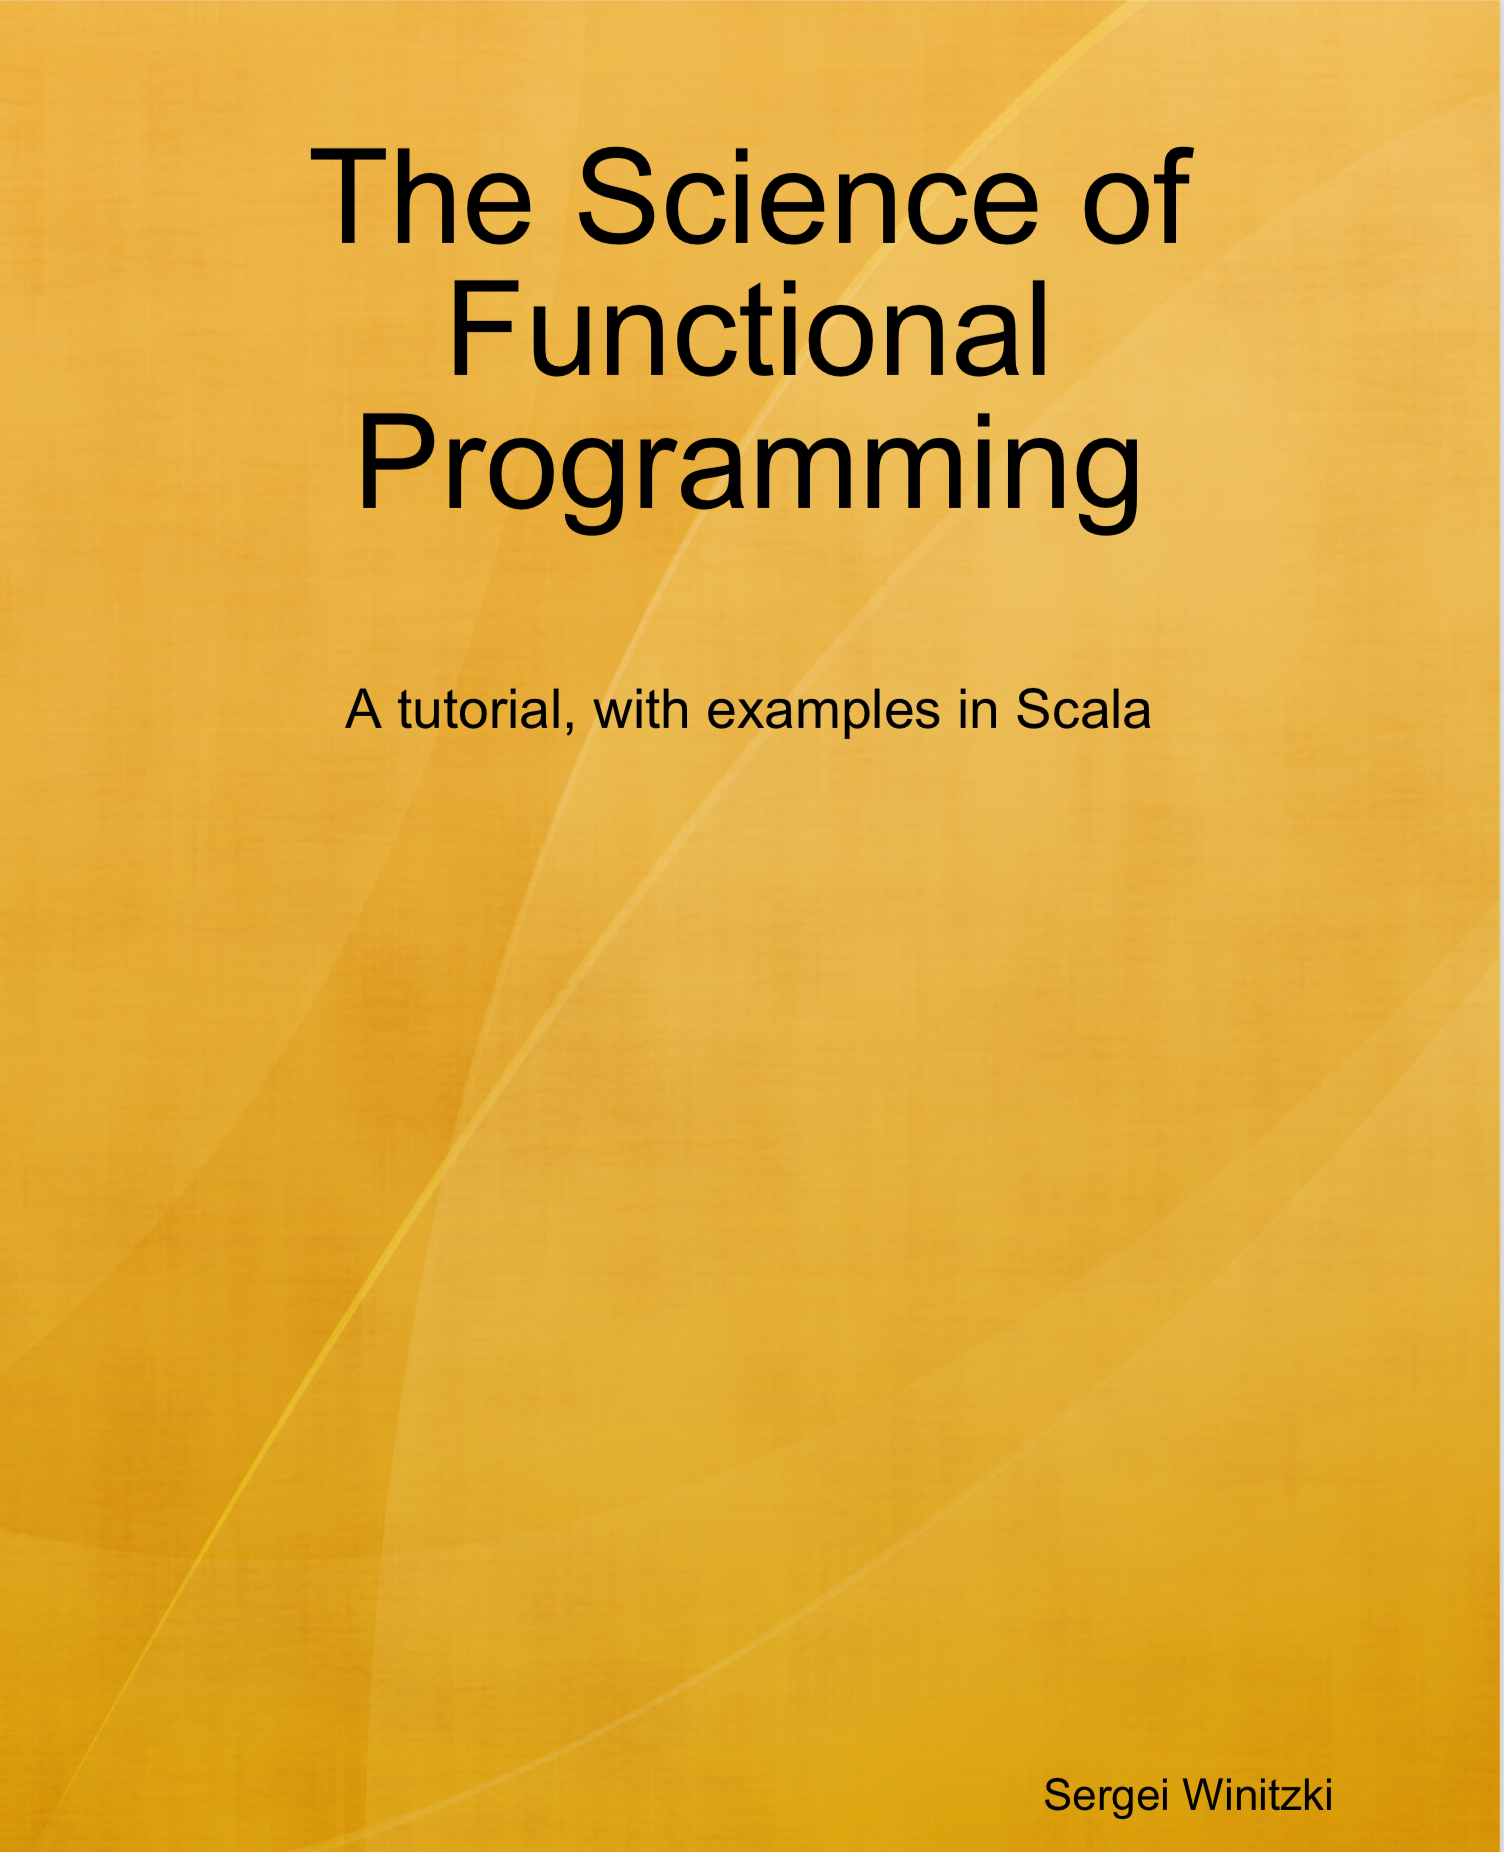
\includegraphics[width=2.5cm]{book-draft-cover}%
\end{minipage}{\small\par}
\par\end{center}

\end{frame}

\end{document}
